\section{Data distribution service for real-time systems}

\subsection{layers in DDS}

There are two sections for the specification of DDS, which are the \textbf{Data Local Reconstruction Layer (DLRL)} and the \textbf{Data Centric Publish Subscribe (DCPS)}.

\subsubsection{Data Local Reconstruction Layer}
DLRL is the upper layer part of the specification that outlines, how an application can interface with DCPS data fields through their own object-oriented programming classes. DLRL is an optional layer within the DDS specification.

Application developers can:
\begin{itemize}
\item describe classes with their methods, data fields, and relations.
\item attach some of those data fields to DCPS entities.
\item manipulate these objects (i.e., create, read, write, delete) using native language constructs
\item activate attached DCPS entities to update objects
\item have these objects managed in a cache
\end{itemize}

\subsubsection{Data Centric Publish Subscribe}	
DCPS is the lower layer API that an application can use to communicate with other DDS-enabled applications.
DCPS is comprised of the following primary entities:
\begin{itemize}
\item Domain
\item Domain Participant
\item Data Writer
\item Publisher
\item Data Reader
\item Subscriber
\item Topic
\end{itemize}

\begin{figure}[ht!]
\centering
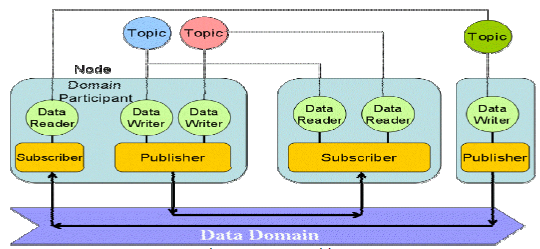
\includegraphics[width=80mm]{img/DDS_Entities.png}
\caption{DDS Entities}
\label{DDSEntities}
\end{figure}

\emph{Data is sent and received from the data domain. Publishers and Subscribers are used to manage
single or multiple Data Writers and Data Readers, respectively. A Data Reader and Data Writer
must be associated to the same Topic if data published by the Data Writer is to be received by the
subscribing Data Reader.}
	
\subsection{The roles of the DDS/DCPS entities}
There are certain roles in the DDSD/DCPS entities - a few are briefly described\footnote{more about this can be read in [1]}:

\begin{description}
\item[Subscriber and Reader] \hfill \\
A Subscriber is an object responsible for receiving published data
and making it available to the application.
To access the received data the application must use a typed DataReader

\item[Publisher and Writer] \hfill \\
A Publisher is an object responsible for data distribution.
A DataWriter object acts as a typed accessor to the publisher.
The application use the DataWriter to communicate a data-object of a given type.

\item[Topic name, type, and key] \hfill \\
A Topic consists of a name and a type - A DDS Topic is the connection between publishers and subscribers.
Name is a string uniquely identifying the topic in a domain.
Type is the definition of the data contained in the Topic.
Keys are for sorting/filtering incoming data
\end{description} 